\chapter{Sviluppi futuri}
\label{cap:sviluppi-futuri}
\emph{In questa sezione vengono proposti alcuni sviluppi futuri del sistema.}
\section{Analisi del contenuto della mail}
Per poter analizzare il contenuto della mail ed estrarre le informazioni associate si può modificare la funzione lambda \textit{processEmail} in modo tale da estrarre il testo della mail e non solo gli allegati ed eventualmente caricarlo su un altro bucket S3.\\
Inoltre, si può implementare un modello di classificazione di Comprehend per classificare il testo della mail in base al contenuto analogamente a quanto fatto per gli allegati e successivamente estrarre le informazioni associate. 
\section{Aggiunta di nuove categorie}
Si possono aggiungere nuove categorie di classificazione se necessario andando a modificare il modello di classificazione di Comprehend e in particolare il dataset fornito. Inoltre, si possono aggiungere nuove funzioni lambda per l'estrazione delle informazioni associate a ciascuna categoria.
\section{Completamento delle informazioni}
Si possono completare le informazioni mancanti e non estratte nello step 2: information extraction come ad esempio la data, l'importo, il mittente, il destinatario, ecc interrogando il database DynamoDB. Questo lavoro si può fare prima dello step 3: human review. 
\subsection{Active learning workflow per migliorare il modello di classificazione}


Si può implementare un workflow di active learning per migliorare il modello di classificazione di Comprehend.

Per avere un riferimento dettagliato si può consultare il seguente link: \href{https://aws.amazon.com/it/blogs/machine-learning/active-learning-workflow-for-amazon-comprehend-custom-classification-part-1/}{Active learning workflow for Amazon Comprehend custom classification}
La figura \ref{fig:active_learning_workflow} mostra un esempio di active learning workflow che utilizza flywheel per migliorare il modello di classificazione di Comprehend.
\begin{figure}[htbp]
  \centering
  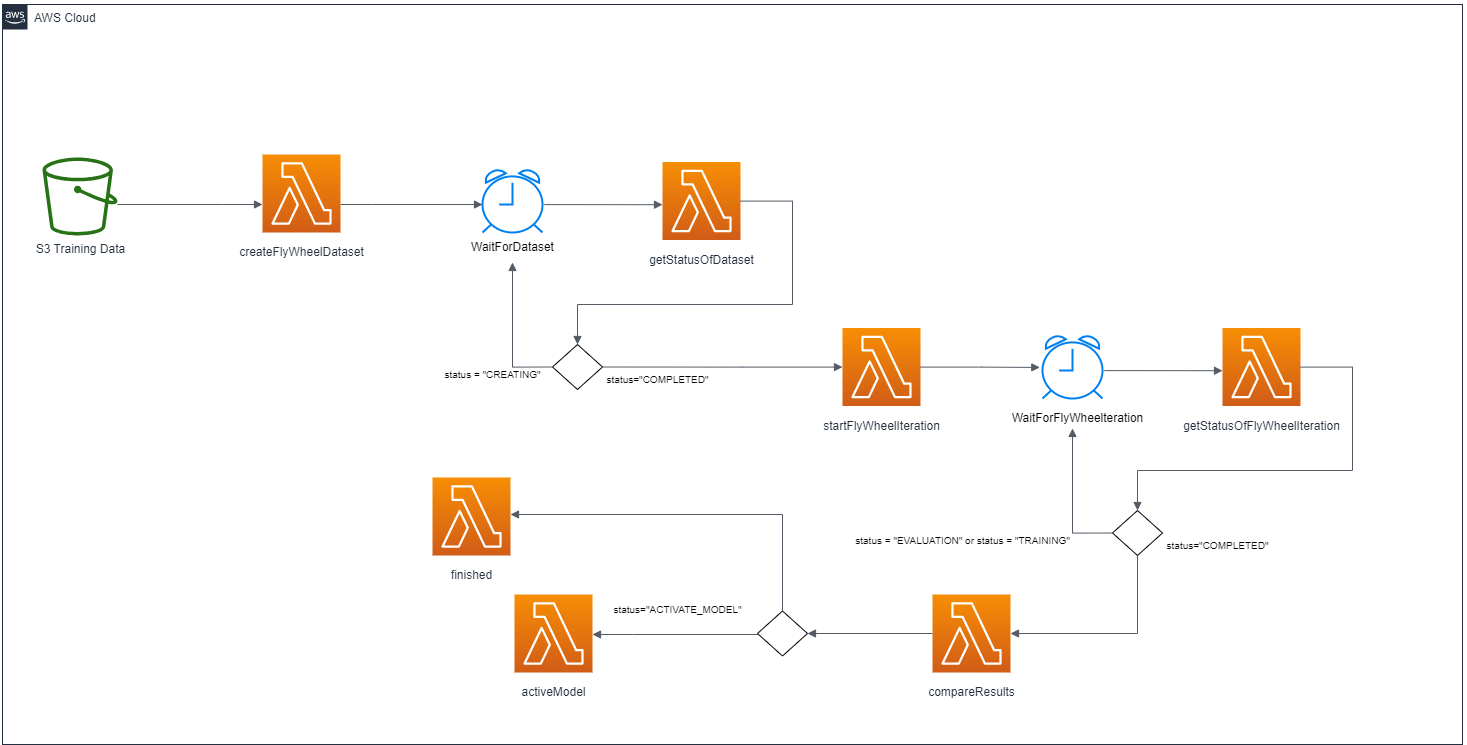
\includegraphics[width=1\textwidth]{img/active_learning_workflow.png}
  \caption{Active learning workflow}
  \label{fig:active_learning_workflow}
\end{figure}
Le sottosezioni successive hanno lo scopo di fornire una panoramica generale su un esempio di active learning workflow per migliorare il modello di classificazione di Comprehend.
\subsubsection{StartStepFunction}
\begin{itemize}
  \item \textbf{Trigger}: L'esecuzione è innescata dalla presenza di un file CSV contenente i dati di training.
  \item Il file CSV viene suddiviso in due file separati: uno per il training e uno per il testing.
  \item Viene avviata la Step Function.
\end{itemize}

\subsubsection{StartCustomClassification}
\begin{itemize}
  \item Viene utilizzata la funzione \texttt{create\_document\_classifier} per creare un classificatore personalizzato.
\end{itemize}
Si attende un periodo di 10 secondi per consentire la creazione del classificatore.

\subsubsection{GetStatusClassifier}
\begin{itemize}
  \item Viene utilizzata la funzione \texttt{describe\_document\_classifier} per ottenere lo stato attuale del classificatore. Gli stati possibili includono \texttt{SUBMITTED}, \texttt{TRAINING}, e altri stati come \texttt{IN\_ERROR}, \texttt{TRAINED}, \texttt{DELETING}, e \texttt{CreateEndpoint}.
  \item Se la variabile \texttt{CurrentClassifierSSM} è impostata, viene restituito lo stato corrente del classificatore.
  \item Se la variabile \texttt{CurrentClassifierSSM} non è impostata:
  \begin{itemize}
    \item Se lo stato è \texttt{TRAINED}, vengono salvate le variabili \texttt{CurrentClassifierSSM}, \texttt{CurrentTrainingDataSSM}, \texttt{CurrentTestDataSSM}, \texttt{CurrentTestingTruthDataSSM} e viene restituito lo stato \texttt{CreateEndpoint}.
  \end{itemize}
\end{itemize}
Nel \textit{choice state}, viene verificato:
\begin{itemize}
  \item Se lo stato è \texttt{TRAINED}, si passa allo stato successivo \texttt{StartValidationTest}.
  \item Se lo stato è \texttt{CreateEndpoint}, si passa allo stato \texttt{StartCustomClassificationEndpointCreation}.
  \item In caso contrario, si attende per 10 secondi e si richiama \texttt{GetStatusClassifier}.
\end{itemize}

\subsubsection{StartValidationTest}
\begin{itemize}
  \item Viene utilizzato il classificatore passato come evento e quello fornito come parametro.
  \item Viene eseguita la funzione \texttt{start\_document\_classification\_job} su entrambi i modelli per classificare i dati di test.
  \item La risposta di entrambi i modelli viene stampata.
  \item Si passa allo stato successivo, trasmettendo l'ID di entrambi i job.
\end{itemize}
Si attende un periodo di 10 secondi per consentire la creazione dei job.

\subsubsection{GetStatusValidationTest}
\begin{itemize}
  \item Viene utilizzata la funzione \texttt{describe\_document\_classification\_job} per ottenere lo stato dei job dei due modelli. Gli stati possibili includono \texttt{COMPLETED}, \texttt{STOP\_REQUESTED}, e altri stati come \texttt{STOPPED}, \texttt{FAILED}.
\end{itemize}
Nel \textit{choice state}, si verifica se lo stato di entrambi i job è \texttt{COMPLETED}. In caso affermativo, si passa allo stato successivo; in caso contrario, si attende per 10 secondi e si richiama \texttt{GetStatusValidationTest}.

\subsubsection{ComputeTestResults}
\begin{itemize}
  \item Vengono scaricati i risultati dei due job (file .gz).
  \item I risultati vengono salvati nella tabella \texttt{TestResultTable} su DynamoDB.
  \item Viene creata una matrice di confusione basata sui risultati e calcolati i parametri di \textit{precision}, \textit{recall}, e \textit{f1-score}.
  \item I parametri vengono salvati nella tabella \texttt{TestResultTable}.
  \item Viene effettuato un confronto su un parametro selezionato:
  \begin{itemize}
    \item Se il vecchio modello risulta migliore, viene restituito lo stato \texttt{DONT\_CREATE}.
    \item In caso contrario, vengono aggiornate le variabili \texttt{CurrentClassifierSSM}, \texttt{CurrentTrainingDataSSM}, \texttt{CurrentTestDataSSM}, \texttt{CurrentTestingTruthDataSSM} con i valori del nuovo modello e viene restituito lo stato \texttt{CREATE}.
  \end{itemize} 
\end{itemize}
Se lo stato è \texttt{DONT\_CREATE}, si passa alla lambda \texttt{FINISHED}; altrimenti, si procede alla lambda \texttt{StartCustomClassificationEndpointCreation}.

\section{Combinazione delle custom queries con analyze expense}
Si può combinare l'uso delle custom queries con analyze expense per migliorare l'estrazione delle informazioni associate a ordini e fatture. In particolare, si può confrontare la percentuale di correttezza delle informazioni estratte con l'uso di queste due funzionalità.

\section{Sviluppo di un'interfaccia grafica}
Invece di caricare manualmente gli allegati o le email nel bucket S3, è possibile sviluppare un'interfaccia grafica che consenta l'upload diretto degli allegati e delle email. Questa soluzione semplificherebbe il processo, migliorando l'efficienza e l'usabilità del sistema.

\section{Utilizzo di A2I (Amazon Augmented AI)}

Per migliorare la precisione del modello, è possibile utilizzare Amazon Augmented AI (A2I). Maggiori informazioni sono disponibili al seguente link: \href{https://aws.amazon.com/it/augmented-ai/}{Amazon Augmented AI}.

\section{Integrazione con un Sistema Documentale}

È possibile integrare il sistema con un sistema documentale per l'archiviazione delle email e degli allegati, migliorando la gestione e l'accessibilità dei documenti.

\section{Utilizzo di Amazon OpenSearch Service}

Amazon OpenSearch Service può essere utilizzato per l'indicizzazione delle informazioni in Amazon DynamoDB, facilitando la ricerca delle informazioni. Questo servizio offre un'esperienza di ricerca sicura e scalabile.

\section{Utilizzo di Amazon CloudFormation}

Amazon CloudFormation può essere utilizzato per automatizzare la creazione e la gestione delle risorse AWS, semplificando il processo di provisioning dell'infrastruttura.